\section{Analysis}
\label{sec:analysis}
The charged particle multiplicity is determined by counting tracklets, formed by pairing clusters with a small angular separation from two \intt layers. 
Two analysis approaches have been developed. The first closely follows the tracklet reconstruction methods outlined in the \phobos and \phenix  publications~\cite{PHOBOS:2010eyu,PHENIX:2000owy} and will be referred to as "the combinatoric method". The second is primarily guided by the LHC Run 2 \xexe and Run 3 \pbpb analyses by the \cms Collaboration~\cite{CMS:2019gzk, CMS:2024ykx} and will be referred to as "the closest-match method". Aspects of the analysis which are common to both methods will be discussed jointly, while the approach-specific methods will be introduced and explained separately.

\subsection{Common analysis components}
% When an \intt channel is activated by its interaction with a charged particle, the induced analog signal is transmitted to the FPHX readout chip~\cite{PHENIX_FPHX_cite}, which processes signals from the channels of each silicon block. The FPHX readout chip performs charge integration, signal waveform shaping, discrimination, and digitization. It features a 3-bit analog-to-digital (ADC) converter composed of eight programmable comparators with predefined thresholds set prior to data taking. The amplitude of the shaped analog signal is compared against all comparators, and the digitized signal amplitude is determined by the highest threshold exceeded. Signals with amplitudes below the first comparator’s threshold are discarded. The digitized signals received by the \intt FELIX readout servers~\cite{FELIX_cite} are associated with the Global-Level 1 (GL1) trigger signal, and hits corresponding to the same GL1 trigger are stored in an event. 
% offline event combining and reconstruction

% Data collected by the \intt, \mbd, and \zdc are sychronised and combined offline based on the BCO of the GL1, allowing temporal alignment across detectors.  

% A set of \intt calibrations is implemented to ensure data quality and optimize hit reconstruction. First, a bad-channel mask is generated to identify hot, cold, and dead channels using a data-driven method. The hit rate of each channel in half of a ladder, corrected for its strip length and radius, is binned into a histogram and fit with a Gaussian function. Channels with significantly higher or lower hit rates than the majority are categorized as hot and cold channels, respectively, while inactive channels are classified as dead. The channels identified as one of these, approximately 4\% of \intt channels, are excluded from the analysis in both data and simulation. Second, only hits occurring within a $\pm1$ BCO relative to the GL1 trigger are retained to eliminate those from non-trigger bunch crossings. Third, an analog-to-digital conversion (ADC) calibration is applied, mapping the 3-bit amplitude of the recorded \intt hits to the predefined threshold setting of the corresponding comparator.
A set of \intt calibrations is implemented to ensure data quality and to optimize hit reconstruction.
First, hot, cold, and dead channels are identified from the data, accounting for approximately 4\% of all \intt channels, and are excluded from the analysis in both real data and simulation. Second, only hits associated with the triggered beam bunch crossing are retained. Third, an analog-to-digital conversion (ADC) calibration is applied, mapping the recorded \intt hit amplitude to the predefined threshold setting of the corresponding comparator.

After extracting \intt hits, hits are clustered using an adjacency graph. Two \intt hits are considered adjacent if and only if they share the same coordinate in $z$ and have touching edges in the azimuthal ($\phi$) direction. Ideally, these clusters represent the full extent of the energy deposition from a charged particle passing through an \intt layer and contain information about its location, timing, size, and energy. A cluster ADC threshold is applied to exclude single-hit clusters with the minimal hit ADC value, which are predominantly noise. Clusters originating from collision-produced particles typically contain at least one strip with a higher hit ADC value. Additionally, unphysically large clusters, which likely result from a rare saturation issue where an \intt chip only read out a portion of its recorded hits, are removed. The impact of this saturation issue is minimal, affecting approximately $10^{-5}$ of the total reconstructed tracklets.

The definition of tracklets is identical between the two analysis approaches. Clusters originating from a particle track associated with the event vertex exhibit small differences in pseudorapidity, azimuthal angle, and angular separation. These variables are defined as $\DEta = \eta_{\text{inner}} - \eta_{\text{outer}}$, $\DPhi = \phi_{\text{inner}} - \phi_{\text{outer}}$, and $\DR=\sqrt{(\Delta\eta)^2 + (\Delta\phi)^2}$.
Here, $\eta_{\text{inner(outer)}}$ and $\phi_{\text{inner(outer)}}$ represent the pseudorapidity and azimuthal angle of the cluster in the inner (outer) layer of the \intt, calculated with respect to the event vertex unless specified otherwise. Both vertex reconstruction and tracklet counting utilize the fact that tracklets associated with particles originating from the event vertex produce a coincidence peak in the $\DEta$, $\DPhi$, and $\DR$ distributions.

The two analyses diverge in the event vertex determination, tracklet reconstruction and counting, and the correction factors, which are discussed separately in the following subsections. The position of the event vertex in the x and y directions is determined by the beamspot, defined as the average vertex position in the transverse plane over multiple events, and the vertex position along the z-axis, referred to as the z-vertex hereafter, which is determined on an event-by-event basis. The transverse vertex position varies by $\mathcal{O}(100)\mum$, which is several orders of magnitude smaller than the length scale of the radial distance between the \intt ladder and the beamline. In contrast, the z-vertex variation is significantly larger, approximately 9.4\cm. 
Determining the z-vertex on an event-by-event basis is crucial for accurately establishing the tracklet kinematics. This is achieved with a reconstruction resolution of 0.17\cm for the selected centrality interval as determined in simulation.

\subsection{The combinatoric method}
Within the combinatoric method, the beamspot position is determined using two techniques: the iterative quadrant search and the two-dimensional tracklet filling method:  

\begin{itemize}
    \item \textbf{The iterative quadrant search}. A bounded square region in the transverse plane, centered at the origin of the \sphenix coordinate system, is defined. The four corners of the square serve as initial beamspot candidates. For each tracklet candidate, $\phi_{\text{inner}}$, $\phi_{\text{outer}}$, $\DPhi$, and the distance-of-closest-approach (DCA) are calculated relative to the candidate position. 
    The correlations between DCA and $\phi_{\text{inner}}$, and between $\DPhi$ and $\phi_{\text{inner}}$ are fitted to a constant function, utilizing the fact that deviations from a horizontal line indicate an incorrect beamspot assumption. 
    The quadrant containing the candidate with the smallest fit uncertainty is selected for the next iteration, where its four corners serve as new beamspot candidates. This iterative process continues until the search window is reduced to a size comparable to the spatial resolution of \intt strips.
    \item \textbf{The 2-dimension tracklet filling method}. The trajectories of cluster pairs are populated into a finely segmented two-dimensional histogram. The beamspot position is obtained as the mean value of the bins with a content exceeding 70\% of the maximum bin content.
\end{itemize}
The iterative quadrant search determines the beamspot position along the x- and y-axes as ($x^{\text{iterative}}_{\text{beamspot}}, y^{\text{iterative}}_{\text{beamspot}}) = (-0.019, +0.230)$\cm, while the 2D tracklet filling method yields ($x^{\text{2-d}}_{\text{beamspot}}, y^{\text{2-d}}_{\text{beamspot}}) = (-0.025, +0.215)$\cm. The final beamspot position used in the analysis of the combinatoric method is determined as the arithmetic mean of both measurements.
  
The $\phi_{\text{inner}}$ and $\phi_{\text{outer}}$ values are updated based on the measured beamspot. For each cluster pair in a given event, a trapezoidal probability distribution is constructed by projecting all possible trajectories that could connect the clusters while crossing the strip acceptances of both along the beam axis. The trapezoidal distributions from cluster pairs are combined to form a stacked distribution. The z-vertex is determined as the average of the mean values from Gaussian functions fitted to the distribution with different fit ranges.

\begin{figure}[t!]
  \centering
  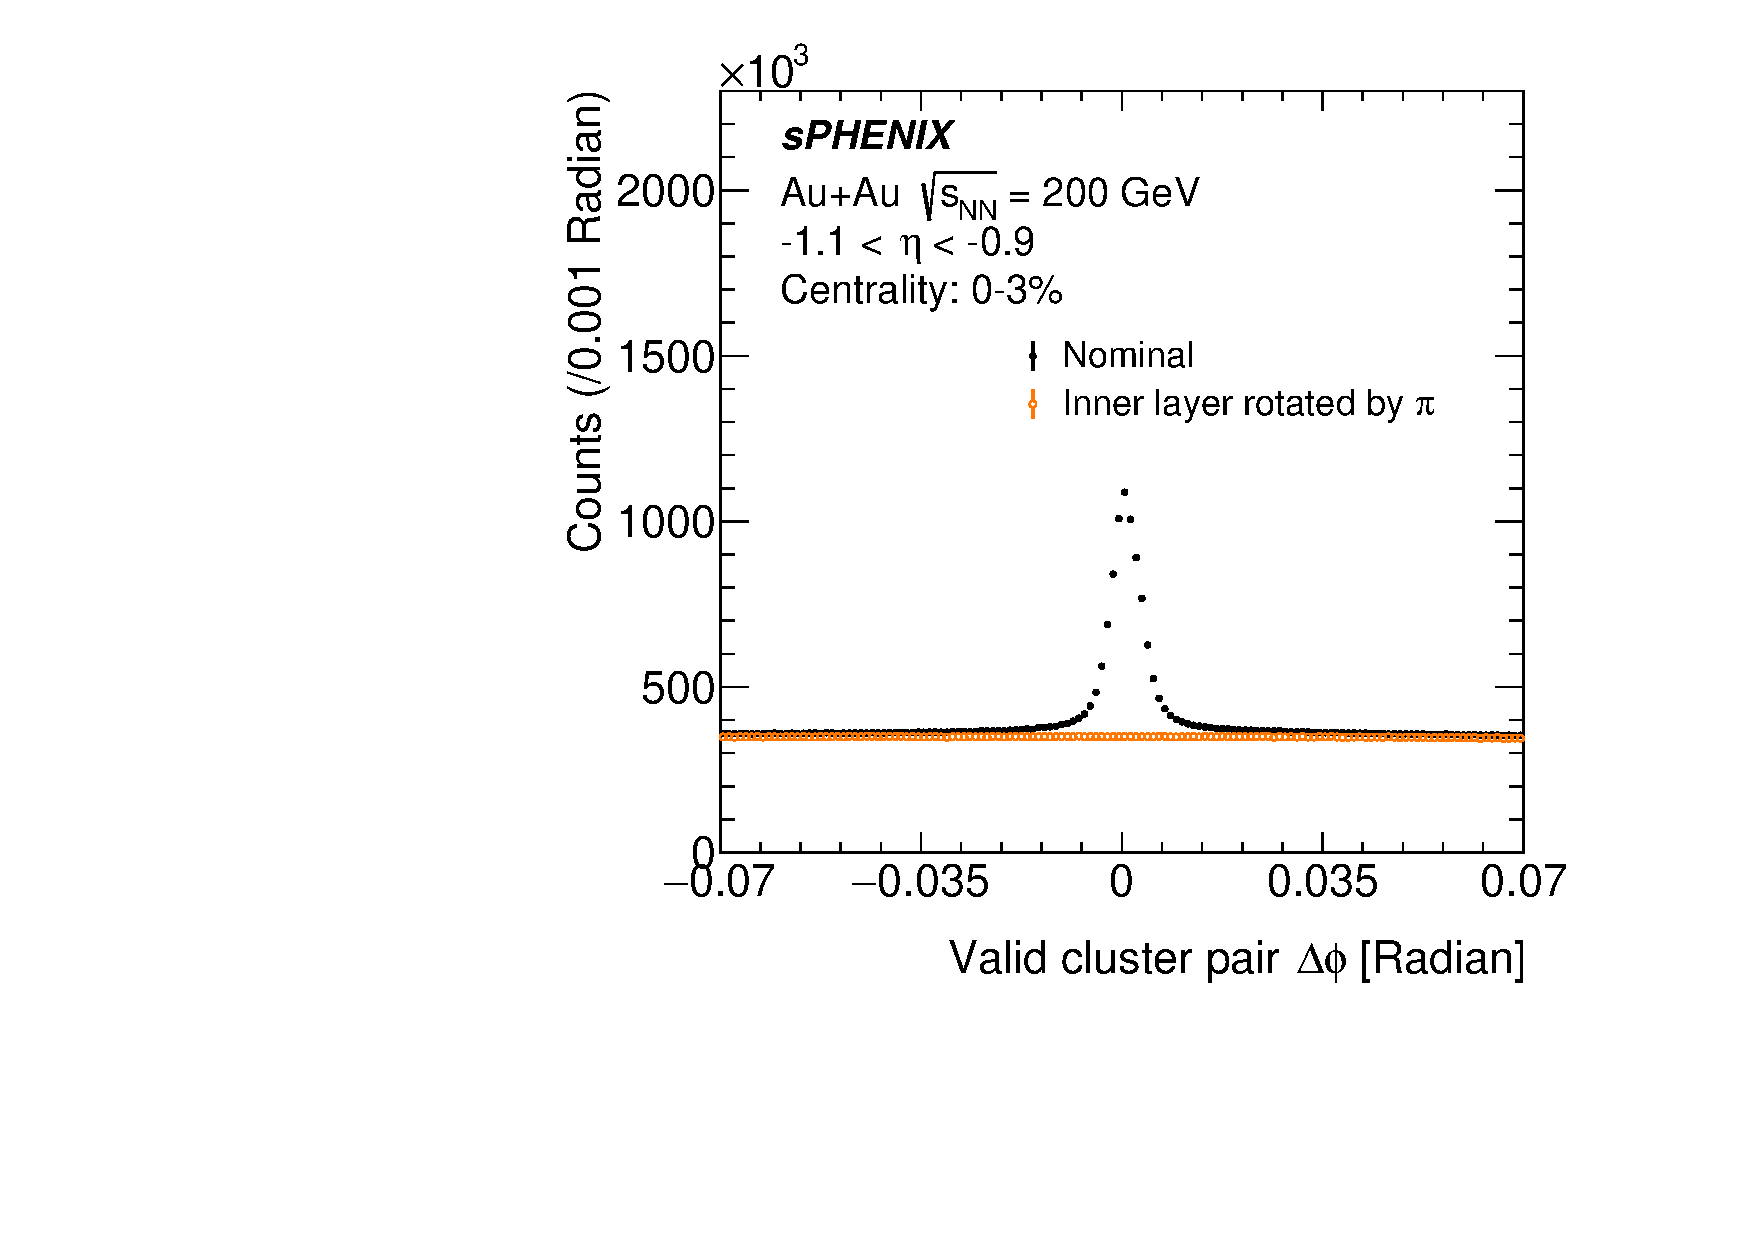
\includegraphics[width=0.5\textwidth]{fig/c1_hstack1D_DeltaPhi_Eta8_sPH.pdf}
  \caption{The $\Delta\phi$ distributions for valid cluster pairs in a representative $\eta$ and centrality interval. The solid black circles indicate the distribution of all valid cluster pairs, while the open orange circles represent the estimated combinatorial background, obtained by rotating the inner-layer ladders by $\pi$ around the beam axis.}
  \label{fig:PHOBOS_deltaphi}
\end{figure}

The $\eta$ values of clusters are recalculated with respect to the estimated z-vertex. Candidate cluster pairs are formed from all possible associations of clusters in the inner layer with those in the outer layer. Clusters are not restricted to a single cluster pair. Valid cluster pairs are defined as those whose trapezoidal projections intersect the reconstructed vertex position. The combinatorial background is estimated by repeating the same pairing procedure after rotating the inner layer by $\pi$ in $\phi$, as illustrated in Figure~\ref{fig:PHOBOS_deltaphi}. This background component is then subtracted from the number of valid cluster pairs. The contribution of combinatorial background is strongly dependent on cluster multiplicity, ranging from 88.4\% in the most central events to 27.0\% in the most peripheral events. The number of reconstructed tracklets within a given $\eta$ and centrality interval is obtained by counting the remaining valid cluster pairs with $|\DPhi|<\text{0.026}$ radians. This $\DPhi$ cut effectively suppresses contributions from particles with $p_T < 50\mev/\text{c}$, including those from two-photon production of dilepton pairs.   

The corrections, derived from simulation, account for the difference between the number of charged hadrons produced in collisions and the number of combinatorial-corrected tracklets, considering acceptance and efficiency losses. For each centrality interval, an $\eta$-dependent correction factor is defined as the ratio of the average number of reconstructed tracklets to the average number of charged hadrons. Within the measured centrality intervals, the correction factors range from 0.8 to 1.0 for $|\eta|<1.1$. These corrections are then applied to the data to obtain the measured \dndeta.

\subsection{The closest-match method}
\label{sec:analysis-closest}
The beamspot position is determined using the DCA-$\phi$ fitting method, closely following the approach developed by the \cms experiment~\cite{Miao:2007zz}. This approach takes advantage of the fact that, for tracks originating from a beamspot at $(x_0,y_0)$, the DCA to the origin exhibits a sinusoidal pattern with respect to the $\phi$ coordinate of the point-of-closest-approach (PCA) to the origin ($\phi_{\text{PCA}}$):
\[
\text{DCA}(\phi_{\text{PCA}})=R_0\cos(\phi_{\text{PCA}}-\phi_0)
\]
where $R_0 = \sqrt{x_0^2 + y_0^2}$ is the radial coordinate of the beamspot, and $\phi_0 = \arctan\big(\frac{y_0}{x_0}\big)$ represents its $\phi$ coordinate. By fitting the sinusoidal pattern formed by the tracklet DCA and $\phi_{\text{PCA}}$, the parameters $R_0$ and $\phi_0$ are extracted.
The determined beamspot position in the x- and y-axis ($x^{\text{DCA-$\phi$ fit}}_{\text{beamspot}}, y^{\text{DCA-$\phi$ fit}}_{\text{beamspot}})=(-0.029, +0.225)\cm$.

The event z-vertex is reconstructed using the following procedure. First, clusters in the inner layer are paired with clusters in the outer layer, with cluster $\phi$ values calculated relative to the beamspot coordinates. For each pair, a z-vertex candidate is constructed, with its boundaries defined by linearly extrapolating the edges of the cluster pair to a line pointing along the longitudinal direction through the beamspot. The candidate range is then divided into fine segments and filled into a one-dimensional histogram. This histogram is fitted with a Gaussian plus a constant offset, and the mean of the Gaussian component is taken as the reconstructed z-vertex position. 

\begin{figure}[t!]
  \centering
  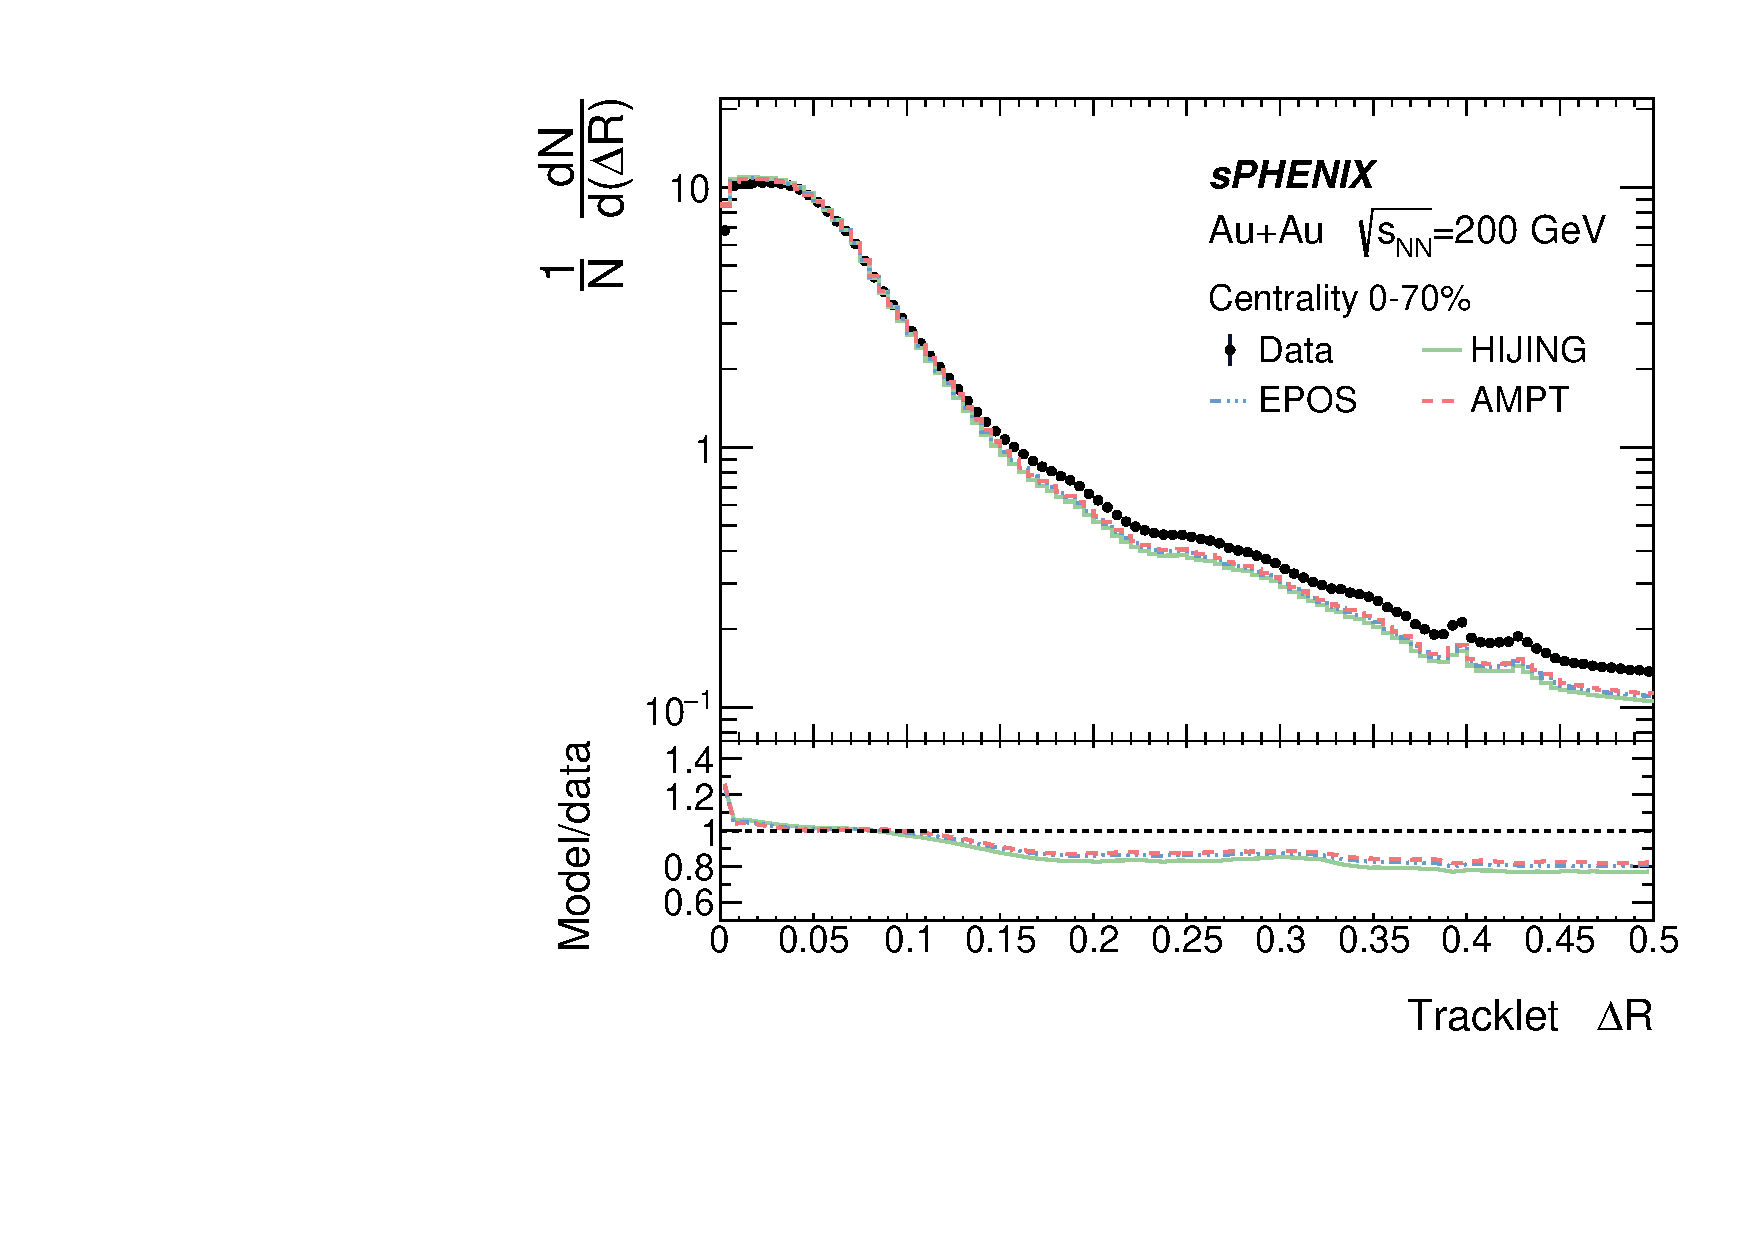
\includegraphics[width=0.5\textwidth]{fig/Paperplot_RecotklDeltaR.pdf}
  \caption{The $\DR$ distributions for reconstructed tracklets, normalised by the total number of tracklets. The spectrum in data (black circle) is compared to simulations generated with \hijing, \epos, and \ampt.}
  \label{fig:recotkldR_approach1}
\end{figure}

Cluster $\eta$ and $\phi$ values are updated relative to the measured beamspot and z-vertex coordinates. Within an event, tracklets are formed by pairing one cluster in the inner barrel with one in the outer barrel. Combinations with $\DR$ less than 0.5 are retained and sorted by $\DR$. This selection criterion ensures that tracklets originating from primary particles are preserved with minimal inefficiency while limiting contamination from secondary particles and combinatorial background to at most 10\%. If multiple matches exist for a cluster, the pair with the smallest $\DR$ is selected to form the final set of reconstructed tracklets. Figure~\ref{fig:recotkldR_approach1} presents the $\DR$ distributions for reconstructed tracklets in data, compared to fully simulated events generated by \hijing, \epos, and \ampt.

Similar to the combinatoric method, the reconstructed tracklet spectrum is corrected to the hadron-level event definition in simulation. In the closest-match method, three multiplicative correction factors are derived and applied. The first compensates for discrepancies between the actual \intt geometry and the geometry implemented in simulations and reconstruction. In simulations, hits are both generated and reconstructed using the same assumed geometry, whereas in real data, minor deviations persist due to detector misalignments that have yet to be implemented in the software geometry. This correction factor is determined by randomly populating tracklets in both data and simulation to estimate the acceptance in the $\eta$ and z-vertex phase space based on tracklet counts and is obtained as the ratio of the tracklet counts from the randomly populated distributions. The correction ranges between 0.9 and 1 for $|\eta|<1.1$.
The second correction, denoted as the $\alpha$ factor, accounts for tracklet reconstruction inefficiencies and is defined as the ratio of primary charged hadrons in simulation to uncorrected reconstructed tracklets. This factor is determined as a function of $\eta$ and z-vertex and applied separately for each centrality interval to correct for efficiency and fake rate variations. The third correction addresses acceptance variations due to shifts in the z-vertex position, which impact tracklet reconstruction near acceptance edges. It is obtained by comparing the total number of tracklets per z-vertex bin to those reconstructed in valid $\alpha$-factor regions and is applied as a function of $\eta$.
The $\alpha$ factor and the acceptance correction are applied jointly, with values ranging between 0.8 and 1.2 for $|\eta|<1.1$.

% The first correction factor accounts for geometric differences between data and simulation. While the \geant geometry is modified based on survey measurements and the software reconstruction geometry is built to match the implemented \geant geometry, neither perfectly replicates the actual \intt geometry in the physical world. As a result, in simulations, hits are generated and reconstructed using the same geometry, whereas in data, hits are recorded at physical locations that deviate from those reconstructed in software. This correction compensates for the resulting discrepancy. To derive this correction factor, each event is assigned a random z-vertex position, uniformly sampled from -10 to 10\cm. Cluster $\eta$ and $\phi$ values are updated accordingly, and "fake" tracklets that do not pass through gaps are reconstructed using the assigned vertex. These tracklets are then binned into a finely segmented histogram in the $(\eta, \text{vtx}_{z})$ space, where bins containing at least one tracklet are set to 1, and empty bins are set to 0. The histogram bins are weighted by the vertex distribution in data and subsequently re-binned into coarser bins. The final correction factor is obtained as the ratio of the simulation histogram to the data histogram. There is no centrality dependence in this correction, as it is purely driven by the detector geometry. $(\eta, \text{vtx}_{z})$ regions where the correction factor falls below 0.75 or exceeds 1.25 are excluded from the analysis. 

% The second correction factor, denoted as the $\alpha$ factor, accounts for tracklet reconstruction inefficiencies and is defined as the ratio of the total number of primary charged hadrons in the simulation to the number of uncorrected reconstructed tracklets. This correction is derived as a function of tracklet $\eta$ and z-vertex and is applied separately for each centrality interval to account for variations in reconstruction efficiency and fake rate due to multiplicity and centrality. Each $(\eta, \text{vtx}_{z})$ bin is required to have an $\alpha$ factor between 0 and 3.6, with a ratio of the $\alpha$ factor to its statistical uncertainty greater than 5. In an ideal scenario where every primary charged hadron is reconstructed as exactly one tracklet, the $\alpha$ factor would be 1. However, when reconstruction inefficiencies occur, leading to fewer reconstructed tracklets than primary charged hadrons, the $\alpha$ factor exceeds 1. Conversely, if fake tracklets are reconstructed without corresponding primary charged hadrons, the $\alpha$ factor falls below 1. In this analysis, typical values of the $\alpha$ factor range between 0.7 and 1.3, with deviations occurring primarily in regions with reduced acceptance.

% The third correction factor accounts for acceptance variations arising from the z-vertex position, as shifts in the vertex position affect the number of reconstructed tracklets near the acceptance edges. To derive this correction, a two-dimensional histogram in $(\eta, \text{vtx}_{z})$ is filled with the total number of tracklets per z-vertex bin. A second histogram is then filled with the number of tracklets reconstructed in regions where the $\alpha$ factor is valid. The correction factor is then obtained as the ratio of these two histograms and projected onto the $\eta$ dimension. Within the measurement range of $|\eta|\leqslant1.1$, this correction factor varies between 0.97 and 1.